
\documentclass[fleqn,12pt]{article}

\usepackage[margin=15mm]{geometry}
\usepackage[utf8]{inputenc}
\usepackage[bulgarian]{babel}
\usepackage[unicode]{hyperref}
\usepackage{amsfonts}
\usepackage{amssymb}
\usepackage{enumitem, hyperref}
\usepackage{indentfirst}
\usepackage{graphicx}
\usepackage{multicol}

\graphicspath{ {./diagrams/} }

\title{Тема 19\\Инженеринг на софтуерните изисквания.Техники за извличане, анализ и валидиране на софтуерните изисквания. Специфициране на изискванията.}

\author{v0.5}
\date{1 юли 2021}

\begin{document}

\maketitle

\tableofcontents

\clearpage

\section{Цели и задачи на инженеринга на софтуерните изисквания}
\textbf{D: Софтуерно изискване} - условие или способност, което трябва да има системата, или е необходимо на потребителя и документалното представяне на условието или способността.

\textbf{D: Процес на инженеринг на изискванията} - систематичен процес на идентифициране, анализиране, документиране и валидиране на функционалностите и ограниченията на даден софтуер, които са изисквани от клиента.

\subsection{Какво правят инженерите по изискванията?}

\begin{itemize}
	\item Изявяват се в началото на проекта
	\begin{itemize}
		\item Идентивицират проблеми, които се нуждаят от решения
		\item Анализът на изискванията е агент на промяната
	\end{itemize}

	\item Инженерите на изискванията трябва да:
	\begin{itemize}
		\item Идентифицират проблема/възможността
		\item Да станат/бъдат експерти в проблемната област
	\end{itemize}

	\item Те трябва да си взаимодействат с други субекти на организацията на процеса (Product management, маркетинг, т.н.)

	\item Фокусът е в дейности по търсене и записване на информацията
\end{itemize}


\subsection{Дейности на процеса на ИИ}

\begin{itemize}
	\item Извличане на изискванията - чрез консултации със ЗЛ
	\item Анализ на изискванията и преговори на изискванията - преговорите са за решаване на конфликти
	\item Документиране на изискванията
	\item Валидиране на изискванията - проверява се за съгласуваност и пълнота
	\item Управление на изискванията - успореден с всички изброени горе, управлява промените в изискванията.
\end{itemize}

\section{Видове изисквания - класификация}

\subsection{Класификация според нивото на детайлност на описанието}

\begin{itemize}
	\item Изисквания на клиента и бизнес изисквания. Съмървил ги дефинира като потребителски изисквания.
	\item Системни изисквания.
	\item Спецификация на софтуерните изисквания.
\end{itemize}

\subsubsection{Бизнес изисквания}
\textbf{D: Бизнес изисквания} - целите на системата от високо ниво на организацията или клиента, които е поръчал системата. Те дефинират визията и обхвата на системата.

Има 2 вида бизнес изисквания - същински бизнес изисквания и изисквания за продукта.

\paragraph{}
\textbf{D: Същински бизнес изисквания} Те представляват резултати (стоки и услуги) от разработката на системата, които ще се предоставят след завършването на системата. Те обслужват бизнес целите чрез:
\begin{itemize}
	\item решаване на проблеми
	\item използване на възможностти
	\item посрещане на предизвикателства
\end{itemize}

\paragraph{}
\textbf{D: Потребителски изисквания} Те описват целите на потребителите и задачите, които потребители трябва да могат да извършат с продукта. Представят  се чрез потребителски случаи, описания на сценарии и таблици със събития и отговори. Те доставят стойност само ако удолетворяват същинските бизнес изисквания.

\subsubsection{Системни изисквания}
\begin{itemize}
	\item Детайлно описание на услугите и ограниченията, което се характеризира с пълнота и консистентност.
	\item Обикновено съдържа структурни модели
	\item Описва изисквания за продукта като система т.е. описва съществуващите зависимости и връзки
	\item Основа за сключване на договор
\end{itemize}

\subsection{Хоризонтална класификация}

\begin{itemize}
	\item Функционални изисквания
	\item Нефункционални изисквания (качествени изисквания + ограничения)
	\item Изисквания, произтичащи от приложната област
\end{itemize}


\subsubsection{Функционални изисквания}
\textbf{D: ФИ} - описват какви функционалности трябва да предоставя системата на клиенти и/или други системи и необходимото поведение от гледната точка на нужните дейности. В някои случай указват какво \textbf{НЕ} трябва да прави системата.

Те се документират чрез три допълващи се, но частично припокриващи се перспективи:
\begin{itemize}
	\item Перспектива на данните
	\item Функционална перспектива
	\item Перспектива на поведението
\end{itemize}

Описанието не трябва да бъде твърде общо, за да се избегне неяснота, и не трябва да бъде твърде специфично, за да се избегнат обемисти документи.


\subsubsection{Нефункционални изисквания}
\textbf{D: НФИ} - изисквания, които не се отнасят до функционалността на системата. НФИ поставят ограничения върху софтуерния продукт и процеса на разработка и уточняват външните ограничения, с които трябва да е съобразен продуктът. Те се отнасят до системата като цяло, а не до някоя отделна функционалност. Състоят се от качествени изисквания и ограничения (организационни изисквания).

\bigbreak
\textbf{Качествени изисквания}
\bigbreak
\textbf{D: Качествени изисквания} - изискванията трябва да описва някаква качествена характеристика, която софтуерната система трябва да притежава като поведение. Например: кратко време за отговор, висока надежност, т.н.

Видове качествени изисквания:
\begin{itemize}
	\item Наличност - процент от времето, през което системата е налична и работи изцяло
	\item Ефективност - мярка за това колко добре системата използва хардуерните си ресурси
	\item Гъвкавост - колко усилия са необходими да се разшири системата с нови възможности
	\item Цялостност -  колко добре е защитена срещу непозволен достъп, нарушаване поверителността на данните, загуба на информация и заразяване с вреден софтуер
	\item Съвместимост - колко лесно системата може да обменя данни с други системи
	\item Надеждност - способността една система да извършва своите функции при указаните условия за определен период от време
	\item Устойчивост - способността една система да продължи да функционира, когато трябва да се справи с определени входни данни, нарушения в свързаните системи или непредвидени условия за работа
	\item Използваемост - усилията, изисквани от потребителите за да подготвят входни данни, да изпозват системата и да интерпретират изходните данни
	\item Възможност за поддръжка - доколко е лесно да се поправи недостатък или да се направи промяна в системата
	\item Преносимост - усилията за извършване на миграция на системата или компонент от една ОС в друга.
	\item Възможност за повторно използване - доколко един компонент може да се ползва в система, за която не е бил разработван първоначално.
	\item Възможност за тестване - степента на леснота, с която софт. компоненти или цялата система могат да се тестват за откриване на дефекти/недостатъци
\end{itemize}

\textbf{Организационни изисквания}

\bigbreak
\textbf{D: Ограничения} - представляват организационно или технологично изискване, което определя начина, по който ще бъде разработена системата.

\bigbreak
\textbf{D: Организационни изисквания} - изисквания, които са ограничения върху процеса на разработка, зависещи от съществуващи политики и процедури в организациите на разработчиците и на клиентите. Те биват 3 вида

\begin{itemize}
	\item Методи и стандарти, които трябва да се следват.
	\item Изисквания за имплементация - език за програмиране, метод за проектиране, технология за разработка, т.н.
	\item Изисквания по доставянето - срокове и отчети, които трябва да бъдат доставени
\end{itemize}

\textbf{Външни изисквания}
\bigbreak
\textbf{D: Външни изисквания} - те са резултат на фактори, външни за системата и за процеса на създаването ѝ. Те могат да са наложени както върху продукта, така и върху процеса на разработване. Това са неща като необходимостта да работи с други системи, съобразяване с правила, закони и корпоративни политики.


\subsubsection{Изисквания, произтичащи от приложната област}
\textbf{D: ИППО} - дефинират се изисквания, резултат от областта на приложение, а не от изискванията на клиента. Тези изисквания могат да бъдат ФИ и НФИ. Тези изисквания произлизат от приложната област на системата, или от основните природни закони.


\section{Същност на отделните етапи на инженеринга на изискванията}

\subsection{Извличане на изискванията}
\textbf{D: Извличане на изискванията} - процес на търсене и откриване и обобщаване на софтуерните изисквания от наличните източници. Включва работа с клиентите за да може да се проучи приложната област и внимателно да се анализират изискванията на ЗЛ.

Дейности по идентифицирането на изискванията:
\begin{itemize}
	\item Разбиране на приложната област - знания за областта в която се прилага системата
	\item Разбиране на проблема - детайлите за специфичния клиентски проблем
	\item Разбиране на бизнеса - как си взаймодействат системите и как спомагат за общите изисквания
	\item Разбиране на нуждите и ограниченията на ЗЛ
\end{itemize}


\subsection{Анализ на изискванията}
\textbf{D: Анализ на изискванията} - целта е да се открият проблеми като незавършеност и несъгласуваност в идентифицираните изисквания, както и да се обсъдят и разрешат със ЗЛ в процеса на преговорите. Той е зависим от опита и експертизата на хората, които са включени в процеса на анализа.

Какво проверява анализа:
\begin{itemize}
	\item Проверка за необходимост - анализира се необходимостта на изискването за да не допуска изисквание, което не допринася за постигането на бизнес целите.
	\item Проверка за съгласуваност и завършеност - прави се cross-check проверка.
	\item Проверка за осъществимост - изискванията се проверяват за това дали са изпълними в контекста на бюджета и плана за разработването на системата.
\end{itemize}


\subsection{Документиране на изискванията}
\textbf{D: Специфициране на изискванията} - Процесът на записване на потребителските и системните изисквания в документ на изисквания.
\begin{itemize}
	\item Изискванията на потребителите трябва да бъдат разбираеми от крайните потребители и клиентите, които нямат техническа подготовка.
	\item Системните изисквания са по-подробни изисквания и могат да включват повече техническа информация.
	\item Системните изисквания могат да бъдат част от договор за разработване на системата.
\end{itemize}

Независимо от използвания език и метод на работа, три аспекта трябва да бъдат документирани за функционалността.
\begin{itemize}
	\item Данни - как са използват и как са структурирани
	\item Функции - условия за ползване, начин на обработка на входните данни и очаквани резултати
	\item Поведение - следи се динамиката на проявление (синоним на инициятива)
\end{itemize}

Отделно имаме допълнителни аспекти за качеството и за ограниченията.

\subsection{Валидиране на изискванията}
\textbf{D: Валидиране на изискванията} - процес на проверка дали изискванията дефинират системата точно така, както клиента го иска. Това е важен процес, защото поправка на изискванията след доставянето на софтуера би струвало 100 пъти повече от поправка на имплементационна грешка.
\bigbreak
Ако анализът работи със сурови изисквания, директно извлечени от заинтересовани лица, то валидирането работи с крайния чернови вариант на формулираните изисквания (тоест, те са вече договаряни и съгласувани.)

Същност на валидирането:
\begin{itemize}
	\item Удолетворява, че документът, описващ изискванията, е приемливо описание на системата.
	\item Документът на изискванията се проверява за пълнота и последователност, конфликти, двусмислици, съответствие със стандартите, грешки в моделите и технически грешки
\end{itemize}

\subsection{Управление на изискванията}
\textbf{D: Управление на изискванията} - Процес на управление на промените на изискванията на системата.

Главните задачи на управлението на изискванията са:
\begin{itemize}
	\item управление на промените в уговорените изисквания
	\item управление на връзките между изискванията
	\item управление на зависимостите между документа на изискванията и други документи, създадени в процеса на инженеринг на изискванията
\end{itemize}

Изискванията не могат да бъдат управлявани ефективно без да има проследимост на изискванията.

\section{Техники за извличане, анализ и валидиране на изискванията, прилагани в отделните етапи на инженеринга на изискванията}

\subsection{Техники за извличане на изискванията}

\subsubsection{Сценарии, случаи на употреба}
Сценариите са примери от реалния живот за това как може да се използва системата. По-подробно, те са точно определена последователност на взаимодействие между актьора и системата.

Предимства: Много са естествени, обикновено ЗЛ ги ползват спонтанно. Кратките сценарии са много добри за бързо илюстриране на специфични взаимодействия
Недостатъци: Липса на структура, трудно се проверяват за пълнота.

\paragraph{Потребителски случаи}
Потребителските случаи са техника, базирана на сценариите, която идентифицира актьорите в едно взаимодействие и която описва самото взаимодействие. Наборът от потребителски случаи описва всички възможни взаимодействия със системата.

\subsubsection{Интервюта, въпросници, анкети}
Изискванията се обсъждат с различни заинтересовани лица, за да се изгради разбиране за техните изисквания. Интервюиращите трябва да бъдат непредубедени и да не провеждат интервюто с предварително формирани идеи за това какво се изисква. Интервютата се фокусират върху въпроси за:
\begin{itemize}
	\item Бизнес случай за проекта
	\item Функционални изисквания за проекта
	\item Рискове
	\item Ограничения
	\item Заинтересовани лица
\end{itemize}

\subsubsection{Мозъчна атака}
Също познат като brainstorming, това е работа в екип, която предизвиква откриването на знания от всеки участник, което помага при разглеждането на алтернативи и правене на правилни избори.

\subsubsection{Работни срещи}
Анализаторът обединява основните ЗЛ, за да анализира системата и да разработи решението. Ръководителят на срещата поддържа фокусирана дискусия, протоколчик документира дискусията.

\subsubsection{Soft systems methods}
Това не са техники за детайлно идентифициране на изискванията. Те са по-скоро начин да се разбере даден проблем и неговия контекст в организацията

 Етапи на SSM:
\begin{itemize}
	\item Оценка на проблемната ситуация
	\item Описание на проблемната ситуация
	\item Абстрактна дефиниция на системата от избрани гледни точки
	\item Концептуално моделиране на системата
	\item Сравнение модел/реален свят
	\item Идентификация на промяната
	\item Препоръки за действие
\end{itemize}

\subsubsection{Наблюдения и социален анализ}
Етнографът прекарва известно време в наблюдение на хората по време на работа и така си изгражда представа за това как се извършва работата. Етнографията може да се използва за извличане на социални изисквания и някои организационни изисквания. Това е хубаво да се комбинира с други техники, по-конкретно интервюта.

\subsubsection{Прототипиране}
Прототипа е начална версия на системата, която може да се използва за експериментиране. Тази експериментация подпомага изясняването и допълването на изискванията. Прототипите могат да прерастнат в крайни продукти и да изследват проектни решения и алтернативи.

 Особености:
\begin{itemize}
	\item Бързото разработване на прототипа е от висока важност, за да може да бъде наличен в ранния етап на процеса на идентификация.
	\item Прототипа може да се ползва както при извличането, така и при валидирането на изискванията
\end{itemize}


 Подходи за бързо прототипиране
\begin{itemize}
	\item На хартия - създава се хартиен мокъп и се използва за системни експерименти
	\item Wizard Of Oz прототипиране - отговорите на системата за определени входни данни се симулира от човек.
	\item Автоматизирано прототипитане - използва се език от 4то поколение или друга среда за бързо разработване, за да се създаде прототип
	(Бележка: 1во поколение - Машинен код; 2ро - Асембли; 3то - C, C++, Java; 4то - Unix Shell, SQL, MATLAB, R)
\end{itemize}


\subsection{Техники за анализ на изискванията}

\subsubsection{Списък на изискванията}
Списък от ключови и достатъчно общи въпроси за оценка на всчко едно изискване.

Един примерен такъв списък:
\begin{itemize}
	\item Преждевременно проектиране - включва ли изискването предварителна информация за проектирането или реализацията
	\item Обединени изисквания - Може ли едно изискване да се раздели на няколко?
	\item Ненужни изисквания - Дали изискването е козметична добавка, и в действителност не е необходимо.
	\item Използване на нестандартни компоненти - Изискването предполага ли използването на нестандартен хардуер или софтуер?
	\item Следване на бизнес целите - Дали изискването е в съгласие с бизнес целите.
	\item Неяснота на изискванията - Могат ли да се прочетат по различен начин от различни хора?
	\item Реалистичност на изискванията - Изискването реалистично ли е при технологията която използваме.
	\item Възможност за тестване на изискванията - Дали може да се тества от QA инжинерите.
\end{itemize}


\subsubsection{Взаимодействия между изискванията}
Много важна цел на анализа е да се открият взаимодействия между изискванията и да посочи конфликтите и припокриванията между изискванията. Това се прави чрез матрица на взаимодействията, която показва как изискванията си взаимодействат.

\subsubsection{Договаряне на изискванията}
Договарянето на изискванията е процес на обсъждане на конфликтите между изискванията и постигане на споразумение, с което всички ЗЛ са съгласни. Разногласията за изисквания са неизбежни при наличието на много ЗЛ. При планирането на процеса на ИИ е важно да се остави достатъчно време за преговори.

Стъпки
\begin{itemize}
	\item Обсъждане на изискванията - Проблемните изисквания се обсъждат, участващите ЗЛ представят своите възгледи за изискванията.
	\item Приоритизиране на изискванията - Спорните изисквания се приоритизират, за да се идентифицират критичните изисквания и да се подпомогне процеса по вземане на решение.
	\item Споразумение на изискванията - Откриват се решения на проблемите и се уговаря компромисен набор от изисквания.
\end{itemize}

\subsection{Техники за валидиране на изискванията}

\begin{itemize}
	\item Преглед на изискванията - Систематичен ръчен анализ на изискванията 
	\item Прототип - използване на изпълним модел на системата за проверка на изискванията.
	\item Валидиране на модели - Проверка за точността на моделите, представени в спецификацията
	\item Генериране на тестови случаи - разработване на тестове за изискванията
\end{itemize}

\subsubsection{Преглед на изискванията}
Най-често използваната техника за валидиране на изискванията: Формулира се специална група, която да се

\begin{itemize}
	\item запознае с изискванията и да ги анализира
	\item формулира забелязани проблеми
	\item дискутира възможните действия за справяне с проблемите
\end{itemize}

Разходът за прегледа на изискванията би могъл да бъде намален ако се направи предварителна проверка от един човек. Целта е да се минат най-явните пропуски, и когато се дадат на повече хора, да не се налага всички да поправят същите очевидни грешки.

Дейности на прегледа:
\begin{itemize}
	\item Планиране - определя се екип, къководител и протоколчик, избира се време и място за срещите.
	\item Разпространение на документите до участниците в екипа.
	\item Подготовка за прегледа - всеки участник да прочете документа и да набележи открити конфликти, пропуски, отклонения от стандартите и др.
	\item Среща по прегледа - дискутират се коментари и проблеми от отделни участници на екипа и се дефинира набора от възможни за справяне с проблемите
	\item Проследяване на действията - ръководителят на екипа проверява дали формулираните действия са изпълнени
	\item Ревизиране на документа - документа се редактира за да отрази съгласуваните действия
\end{itemize}

\subsubsection{Прототип}
Тази техника се прилага само ако системата има вече разработен прототип. В противен случай времето и средствата загубени в този прототип няма да си струват.

Прототипите имат за цел да демонстрират изискванията и да помогнат на ЗЛ да открият проблеми. Те трябва да бъдат достатъчно пълни, ефикасни и robust, за да се оцени използването на исканата система. Валидирането може да започне с непълен прототип, но задължително системата трябва да бъде допълнена и довършена по време на валидирането.

Действия при прототипизирането:
\begin{itemize}
	\item Избор на подходящ екип за тестване на прототипа - потребители с умерен опит и които са "отворени" към използването на нови системи.
	\item Разработване на тестови сценарии - при внимателното планиране се получава формулиране на достатъчно пълен набор от тестови сценарии.
	\item Изпълнение на сценариите - хубаво е потребителите да ги изпълняват самостоятелно --- по този начин симулират реалната ситуация на използването на системата,
	\item Документиране на проблемите - съставяне на електронен или хартиен документ с откритите проблеми.
\end{itemize}

\subsubsection{Валидиране на модели}

Цел на валидирането:
\begin{itemize}
	\item Проверява дали моделът е логичен, съдържа цялата необходима информация, няма конфликти
	\item Проверява дали моделите за една система са вътрешно и външно съвместими
	\item Проверява дали всеки модел представя реалните изисквания на клиента
\end{itemize}

Някои проверки са възможни с автоматични софтуерни инструменти - CASE

\subsubsection{Тестване на изискванията}
За всяко изискване трябва да може да бъдат съставени тестове за проверка дали изискването е добре дефинирано. Невъзможността да се създаде тест значи, че има липсваща или неясна информация в описанието на изискванията. Всяко функционално изискване в документа трябва да бъде анализирано с подходящ тест.

Няколко въпроса, подпомагащи съставянето на тест за изискванията:
\begin{itemize}
	\item Каква употреба ще се тества?
	\item Съдържа ли изискването достатъчна информация, за да позволи разработването на тест?
	\item Нужен ли е повече от един тест за правене на изследването?
	\item Може ли изискването да бъде преформулирано, за да бъдат тестовите случаи по-ясно дефнирани?
\end{itemize}


Формуляр на тест за изискванията.
\begin{itemize}
	\item Идентификатор на изискването
	\item Свързани изисквания
	\item Описание на теста - да е кратко, да обясни защо тестът е обективен за даденото изискване, описание на входно изходна информация.
	\item Проблеми - описание на проблемите, които правят теста труден или невъзможен
	\item Коментари и препоръки - съвети за евентуални решения на откритите проблеми.
\end{itemize}

\section{Начини за специфициране на изискванията. Видове модели в зависимост от перспективата  на  системата.}
\textbf{D: Модел на процес} - опростено описание на процес, обикновено представен от конкретна перспектива. Моделът отразява или възпроизвежда процеса на изследването в достатъчна степен, за да позволи получаване на информация за неговото изучаване.

\subsection{Модел  на  потока  на  данните}
Също познат като DFM, той представя потока на информация в рамките на системата, както и между системата и средата. Той не показва последователност на поведение и на управляваша информация.

Диаграмата на моделът (DFD) е графично представяне на:
\begin{itemize}
	\item външни за процеса елементи
	\item процеси (функции)
	\item поток на данните
	\item хранилища за данни
\end{itemize}

\begin{multicols}{2}

Елементи на DFD
\begin{itemize}
	\item External Entity - външен източник или получател на данни. Те обикновенно са извън обхвата на изучаваната област.
	\item Process - трансформира или манипулира данни
	\item Data flow - пренася данни между източник и процес, процес и получател или между 2 процеса
	\item Data Store - хранилище на данни
	\item Connector symbols - ползват се в случай, че диаграмата се представя на няколко страници.
\end{itemize}

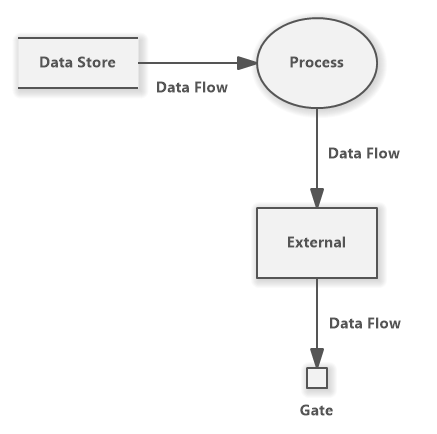
\includegraphics[scale=0.6]{data-flow-diagram}

\end{multicols}

\pagebreak
\subsection{Модел  на  поведението}
State Transition Diagram (STD) - показва динамиката в поведението на една система: Как системата реагира на последователност от външни събития и как независими компоненти координират работата си.

\begin{multicols}{2}

Основни компоненти:
\begin{itemize}
	\item Състояние
	\item Действие/събитие - биват 2 вида
	\begin{itemize}
		\item Външно и/или вътрешно
		\item Времево
	\end{itemize}
	\item Преходи между състоянията
\end{itemize}

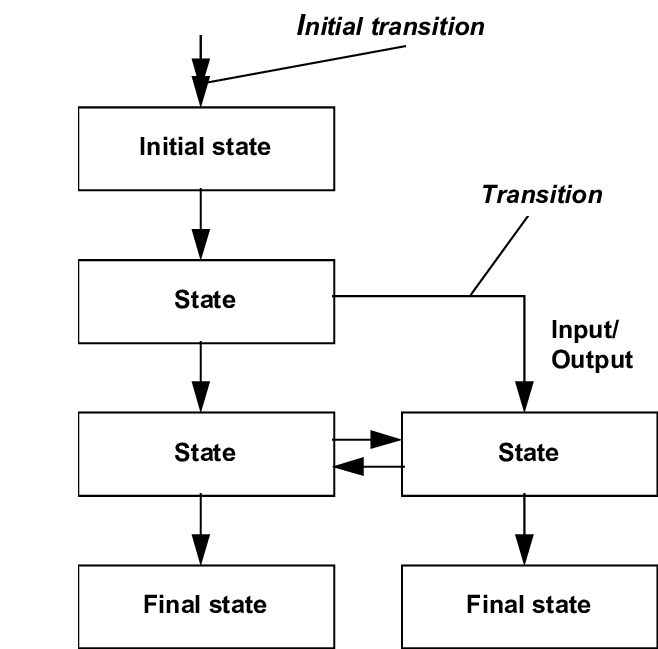
\includegraphics[scale=.25]{std}

\end{multicols}

\subsection{Семантични модели}
Семантичния модел е модел на данните, който представя субектите в база данни, техните атрибути и техните връзки. Описва се чрез Entity Relationship Diagram (ERD), които представят логическия вид на данните и връзките между тях.
\begin{multicols}{2}

Основни компоненти:
\begin{itemize}
	\item Същност (Entity): обект или дейност
	\item Атрибути (Attributes)
	\item Връзки (Relationships) - елементи:
	\begin{itemize}
		\item кардиналност (cardinality): (1:1), (n:1), (1:n), (n:m)
		\item опционалност: задължителна или незадължителна
		\item зависимост
	\end{itemize}
\end{itemize}

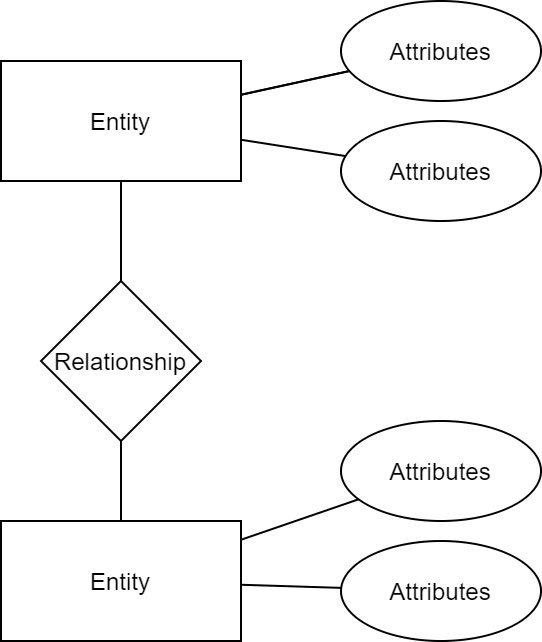
\includegraphics[scale=.33]{ERD}

\end{multicols}

\subsection{Обектно-ориентирани модели}
ООМ представят едновременно данните и тяхна обработка, както и класификация и връзки на субектите на системата. Обектно-ориентираният анализ, проектиране и разработка е общоприет.

Основни концепции на ООМ:
\begin{itemize}
	\item Обект - Нещо, за което запазваме данни и описваме операции за манипулиране на тези данни
	\item Клас - Описание на множество от обекти, които споделят общи атрибути и операции. Обектът е инстанция от класа.
	\item Операции - действие за четене и манипулиране данните на обект. 
	\item Метод - реализация на дадена операция, специфицира се пътя, по който операциите се имплементират.
	\item Капсулиране на данни за обект - Пакетиране на данни и операции, което предпазва данните на обекта от неразрешен достъп
	\item Онаследяване - при таксономия на класовете обекти на по-ниско ниво в йерархията наследяват атрибутите и операциите на техните родители.
	\item Съобщения - начин по които обектите си комуникират. Когато обект получи съобщение, то той извиква операция изпълняваща подходящ метод.
\end{itemize}


\subsection{Формални модели}
ФМ осигуряват високо ниво на точност на системата, която да покрие напълно спецификацията, но не могат да гарантират абсолютна точност. Те са ниво на абстракция, която позволява да се създаде качествен софтуер. 

\begin{multicols}{2}

Основни компоненти:
\begin{itemize}
	\item Синтаксис - специфична нотация за представяне на спецификацията
	\item Семантика - дефинира съвкупността от обекти, които ще се използват, за да се опише системата.
	\item Връзки - дефинират правилата, които показват кои обекти правилно удолетворяват спецификацията.
\end{itemize}

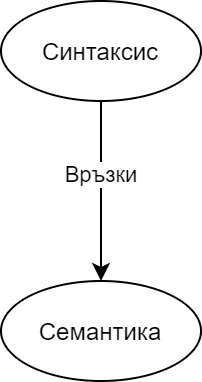
\includegraphics[scale=.4]{FD}

\end{multicols}



\end{document}
